\def\mytitle{CONIC ASSIGNMENT}
\def\myauthor{PANJUGALA SHASHIKALA}
\def\contact{sashipanjugala@gmail.com}
\def\mymodule{Future Wireless Communication (FWC)}
\documentclass[10pt, a4paper]{article}
\usepackage[a4paper,outer=1.5cm,inner=1.5cm,top=1.75cm,bottom=1.5cm]{geometry}
\twocolumn
\usepackage{setspace}
\doublespacing
\usepackage{graphicx}
\graphicspath{{./images/}}
\usepackage[colorlinks,linkcolor={black},citecolor={blue!80!black},urlcolor={blue!80!black}]{hyperref}
\usepackage[parfill]{parskip}
\usepackage{lmodern}
\usepackage{tikz}
	\usepackage{physics}
%\documentclass[tikz, border=2mm]{standalone}
\usepackage{karnaugh-map}
%\documentclass{article}
\usepackage{tabularx}
\usepackage{circuitikz}
\usetikzlibrary{calc}
\usepackage{amsmath}
\usepackage{amssymb}
\renewcommand*\familydefault{\sfdefault}
\usepackage{watermark}
\usepackage{lipsum}
\usepackage{xcolor}
\usepackage{listings}
\usepackage{float}
\usepackage{titlesec}
\usepackage{amsmath}
\providecommand{\mtx}[1]{\mathbf{#1}}
\titlespacing{\subsection}{1pt}{\parskip}{3pt}
\titlespacing{\subsubsection}{0pt}{\parskip}{-\parskip}
\titlespacing{\paragraph}{0pt}{\parskip}{\parskip}
\newcommand{\figuremacro}[5]{
    \begin{figure}[#1]
        \centering
        \includegraphics[width=#5\columnwidth]{#2}
        \caption[#3]{\textbf{#3}#4}
        \label{fig:#2}
    \end{figure}
}
\newcommand{\myvec}[1]{\ensuremath{\begin{pmatrix}#1\end{pmatrix}}}
\let\vec\mathbf
\lstset{
frame=single, 
breaklines=true,
columns=fullflexible
}

\thiswatermark{\centering \put(-15,-100.0){\includegraphics[scale=0.4]{iith.png}} }
\title{\mytitle}
\author{\myauthor\hspace{1em}\\\contact\\FWC22097 -\hspace{0.5em}IITH\hspace{0.5em}\mymodule\hspace{6em}}
\date{}


\begin{document}
\maketitle


\section{Question}
\textbf{\textit{Q(6), C , Section-A, Chapter-8:}The axis of a parabola is along the line y=x and the distance of  its vertex and focus from the origin are $\sqrt{2}$ and $2\sqrt{2}$    respectively. If vertex and focus both lie in the first quadrant, then the equation of the parabola is }

\section{Solution}
\raggedright 

\begin{figure}[h!]
\centering
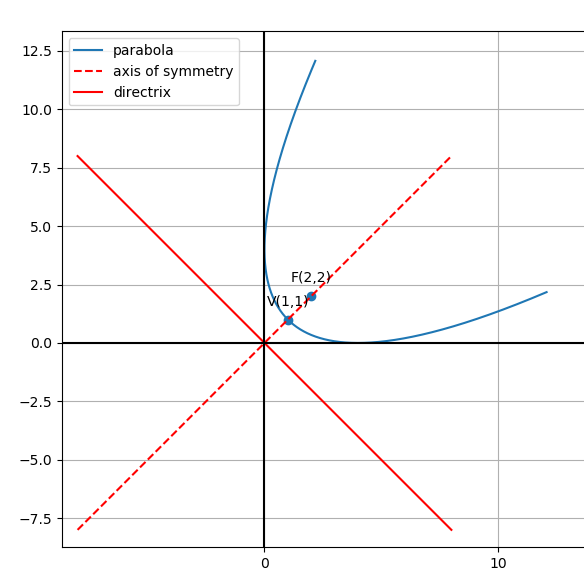
\includegraphics[scale=0.3]{conic.png} \\
\end{figure}

\vspace{0.25cm}
Given the parabola has the axis of symmetry along the line y=x. And focus and vertex lies in first quadrant.\\ The distance from the origin to the vertex is given as $\sqrt{2}$.\\
Let O be the origin,v be the vertex and F be the focus of the parabola.
$$\vec{O}=\myvec{ 0 \\ 0}$$
$$\vec{v}=\myvec{ x \\ y}$$
We can write
$$||\vec{v}-\vec{O}||=\sqrt{2}$$
$$(\vec{v-O})^{\top}(\vec{v-O})=2$$
which can be written as \\
$\implies(\vec{v-O})^{\top}(\vec{v-O})$=
$
\begin{bmatrix}
1 & 1 \\
\end{bmatrix}
$
$
\begin{bmatrix}
1 \\
1 \\
\end{bmatrix}
$ \\

$
\implies\begin{bmatrix}
x & y \\
\end{bmatrix}
$
$
\begin{bmatrix}
x \\
y \\
\end{bmatrix}
$ = 
$
\begin{bmatrix}
1 & 1 \\
\end{bmatrix}
$
$
\begin{bmatrix}
1 \\
1 \\
\end{bmatrix}
$ \\
\vspace{0.5cm}
From the above matrix, we can find x and y values as 
$$\vec{v}=\myvec{ 1 \\ 1}$$

$$||\vec{v}-\vec{O}||=2\sqrt{2}$$
$$(\vec{F-O})^{\top}(\vec{v-O})=8$$

$\implies(\vec{F-O})^{\top}(\vec{F-O})$=
$
\begin{bmatrix}
2 & 2 \\
\end{bmatrix}
$
$
\begin{bmatrix}
2 \\
2 \\
\end{bmatrix}
$ \\

$
\implies\begin{bmatrix}
x1 & y1 \\
\end{bmatrix}
$
$
\begin{bmatrix}
x1 \\
y1 \\
\end{bmatrix}
$ = 
$
\begin{bmatrix}
2 & 2 \\
\end{bmatrix}
$
$
\begin{bmatrix}
2 \\
2 \\
\end{bmatrix}
$ \\
\vspace{0.5cm}
From the above matrix, we can find x1 and y1 values as
$$\vec{F}=\myvec{ 2 \\ 2}$$

Given the axis of symmetry of parabola as x-axis.Therefore,directrix of the parabola will be the line perpendicular to the axis of symmetry i.e, $$ x+y=0 $$
Comparing with the line equation,$$\vec{n}^{\top}x=c$$
$$\vec{n}=\myvec{1 \\ 1}$$
and c=0.\\
By using $\vec{v}$,$\vec{F}$ and $\vec{n}$ values,we can find $\vec{V}$,$\vec{u}$,f values of parabola.\\
The equation of a conic with directrix $\vec{n}^{\top}x=c$, eccentricity e and focus F is given by
\begin{equation}
\vec{x}^{\top}\vec{V}\vec{x}+2\vec{u}^{\top}\vec{x}+f=0
\end{equation}
\begin{equation}
\vec{V}=||\vec{n}||^2I-e^2\vec{n}\vec{n}^{\top}
\end{equation}
Where I=Identity matrix,e=1.\\ 
By substituting I,e,$\vec{n}$ values in equation (2),we get
$$
\vec{V}=
\begin{bmatrix}
1 & -1 \\
-1 & 1\\
\end{bmatrix}
$$
\begin{equation}
\vec{u}=ce^2\vec{n}-||\vec{n}||^2\vec{F}
\end{equation}
By substituting c,e,$\vec{n}$.$\vec{F}$ values in qquation (3),we get
$$\vec{u}=\myvec{ -4 \\ -4 }$$
\begin{equation}
f=||\vec{n}||^2||\vec{F}||^2-c^2e^2
\end{equation}
By substituting c,e,$\vec{n}$.$\vec{F}$ values in equation (4),we get\\
$$f=16$$
\vspace{0.5cm}
By substituting $\vec{V}$,$\vec{u}$ and f values in equation (1),we get the equation of parabola.\\
\vspace{0.5cm}




\section{Software}


The below python code realizes the above construction:	\\
\begin{lstlisting}
https://github.com/PanjugalaShashikala/FWC_2022097/tree/main/Lines
 \end{lstlisting}

\end{document}
